\section{Tavşanlara Karşı Koyunlar}

\begin{justify}
Bu bölümde faz düzlemi analizinin klasik bir örneği olarak iki tür arasındaki rekabet modeli ele alınır. Türler tavşanlar ve koyunlar olarak düşünülür. Her iki türün de aynı sınırlı besin kaynağı için rekabet ettiği varsayılır.

Bu varsayımları içeren Lotka--Volterra tipi model
\begin{align}
\dot{x} &= x(3-x-2y),\\
\dot{y} &= y(2-y-x)
\end{align}
şeklindedir. Burada
\begin{equation}
x(t)=\text{tavşan popülasyonu}, \qquad y(t)=\text{koyun popülasyonu}
\end{equation}
olup $x,y\ge 0$ kabul edilir.

Sabit noktalar $\dot{x}=0$ ve $\dot{y}=0$ denklemlerinin birlikte çözülmesiyle bulunur:
\begin{equation}
(0,0), \qquad (0,2), \qquad (3,0), \qquad (1,1).
\end{equation}
Sınıflandırma için Jacobian matrisi
\begin{equation}
A=\begin{pmatrix}
\dfrac{\partial \dot{x}}{\partial x} & \dfrac{\partial \dot{x}}{\partial y}\\[0.3cm]
\dfrac{\partial \dot{y}}{\partial x} & \dfrac{\partial \dot{y}}{\partial y}
\end{pmatrix}
=
\begin{pmatrix}
3-2x-2y & -2x\\
-y & 2-x-2y
\end{pmatrix}
\end{equation}
olur.

$(0,0)$ noktasında $A=\begin{pmatrix}3&0\\0&2\end{pmatrix}$ olduğundan bu nokta kararsız düğümdür (Şekil~\ref{fig:6-4-1}).
\begin{figure}[H]
\centering
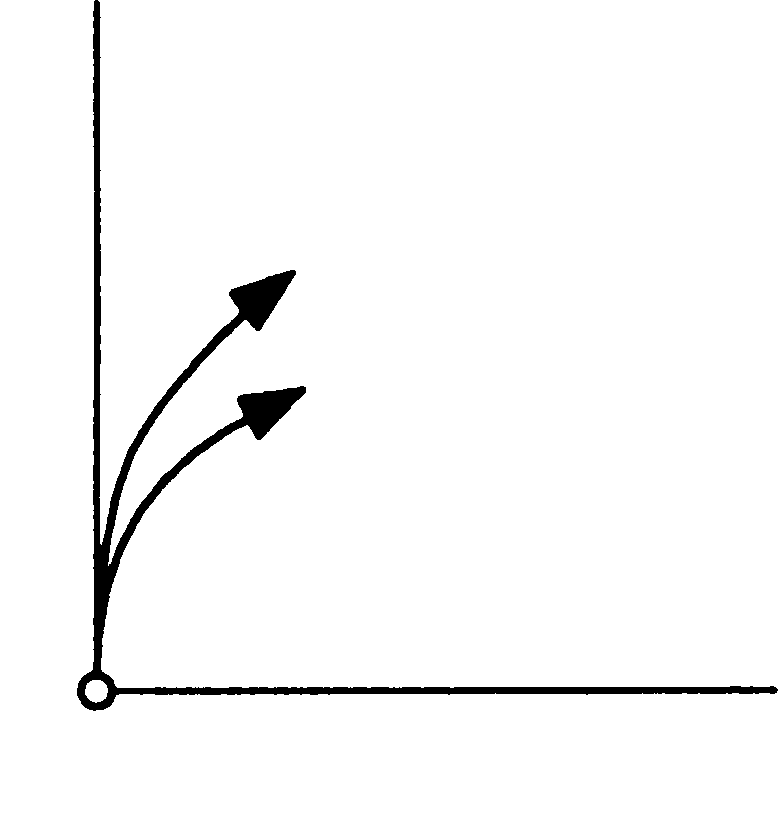
\includegraphics[width=0.82\textwidth]{images/Figures/figur-009.png}
\caption{Tavşan--koyun modelinde $(0,0)$ yakınındaki kararsız düğüm.}
\label{fig:6-4-1}
\end{figure}

$(0,2)$ noktasında $A=\begin{pmatrix}-1&0\\-2&-2\end{pmatrix}$ olduğundan bu nokta kararlı düğümdür (Şekil~\ref{fig:6-4-2}).
\begin{figure}[H]
\centering
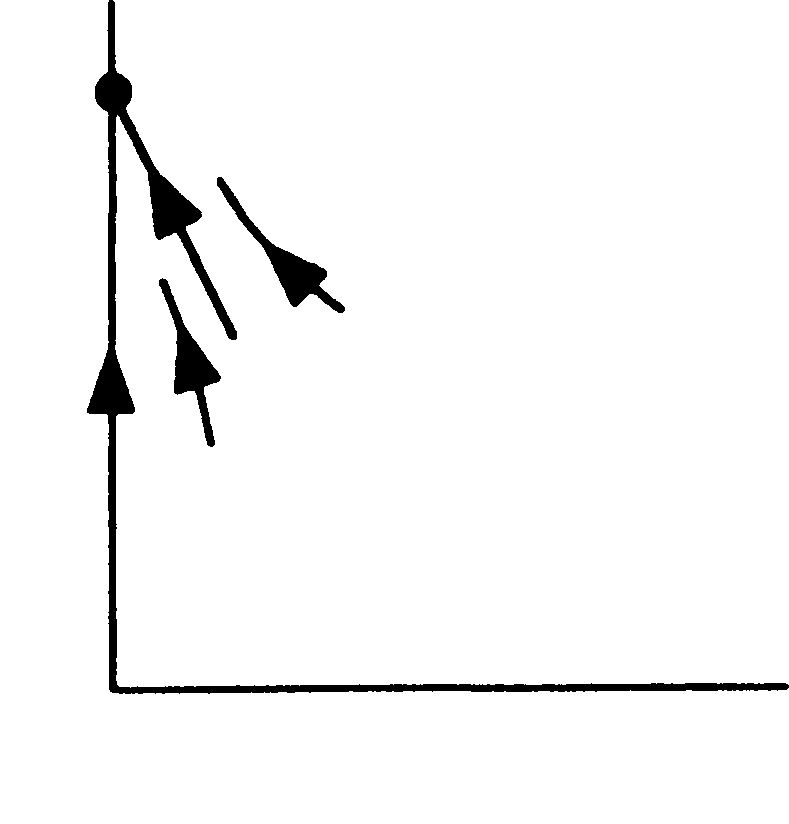
\includegraphics[width=0.82\textwidth]{images/Figures/figur-010.png}
\caption{Tavşan--koyun modelinde $(0,2)$ yakınındaki kararlı düğüm.}
\label{fig:6-4-2}
\end{figure}

$(3,0)$ noktasında
\begin{equation}
A=\begin{pmatrix}-3&-6\\0&-1\end{pmatrix}, \qquad \lambda=-3,-1
\end{equation}
olur. Bu nokta da kararlı düğümdür (Şekil~\ref{fig:6-4-3}).
\begin{figure}[H]
\centering
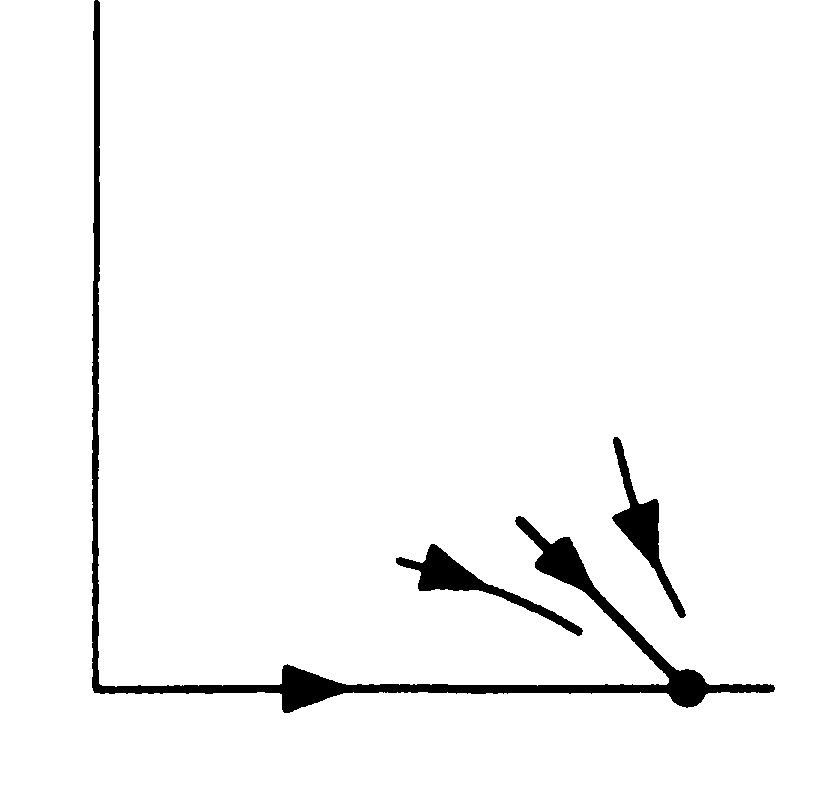
\includegraphics[width=0.82\textwidth]{images/Figures/figur-011.png}
\caption{Tavşan--koyun modelinde $(3,0)$ yakınındaki kararlı düğüm.}
\label{fig:6-4-3}
\end{figure}

$(1,1)$ noktasında
\begin{equation}
A=\begin{pmatrix}-1&-2\\-1&-1\end{pmatrix}, \qquad \lambda=-1\pm\sqrt{2}
\end{equation}
olduğundan bu nokta bir eyer noktasıdır (Şekil~\ref{fig:6-4-4}).
\begin{figure}[H]
\centering
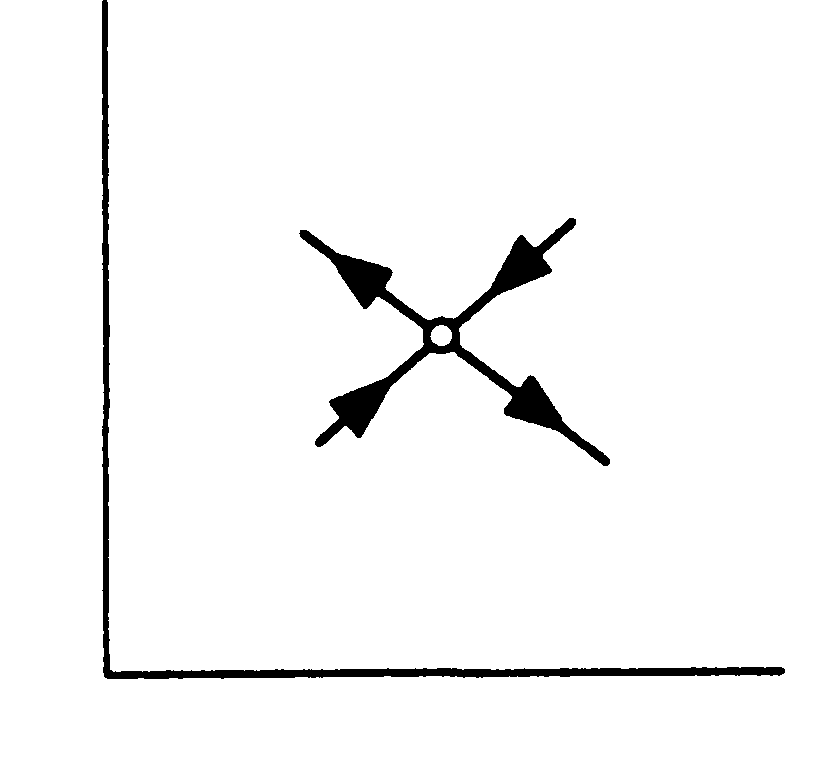
\includegraphics[width=0.82\textwidth]{images/Figures/figur-012.png}
\caption{Tavşan--koyun modelinde $(1,1)$ yakınındaki eyer noktası.}
\label{fig:6-4-4}
\end{figure}

Yerel faz portreleri birleştirildiğinde genel taslak elde edilir (Şekil~\ref{fig:6-4-5}). Eyer noktasına yaklaşan özel yörüngeler eyerin kararlı manifoldunu oluşturur (Şekil~\ref{fig:6-4-6}). Bilgisayar üretimli faz portresi Şekil~\ref{fig:6-4-7}'de gösterilecektir.
\begin{figure}[H]
\centering
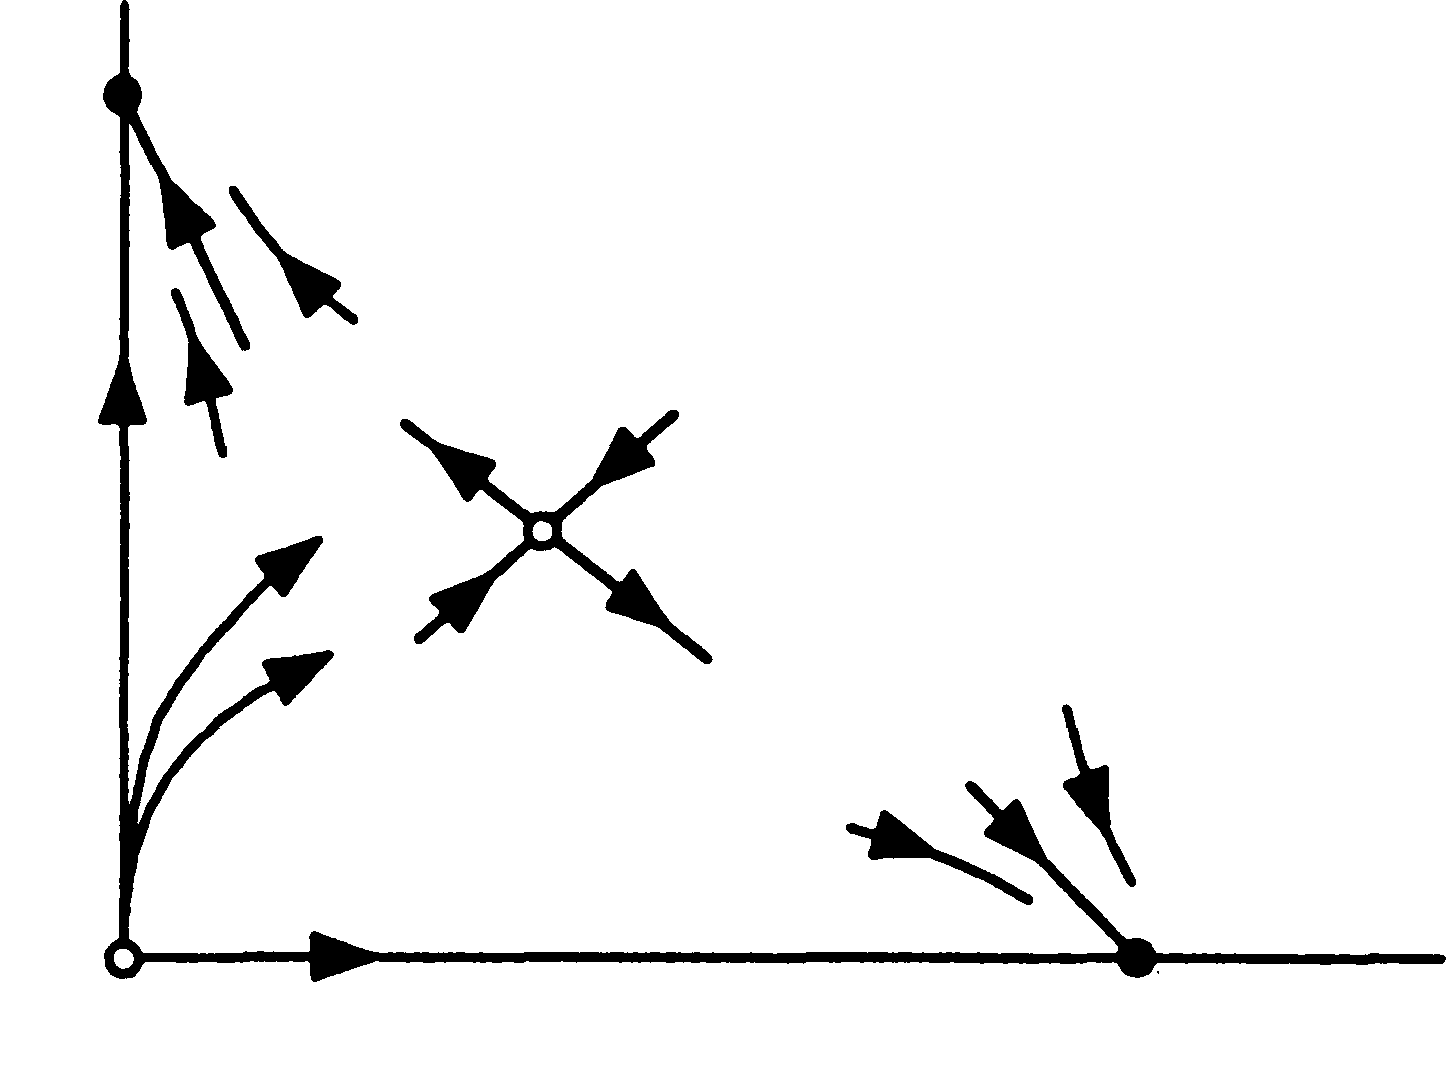
\includegraphics[width=0.82\textwidth]{images/Figures/figur-013.png}
\caption{Yerel faz portrelerinin birleştirilmesiyle elde edilen genel taslak.}
\label{fig:6-4-5}
\end{figure}
\begin{figure}[H]
\centering
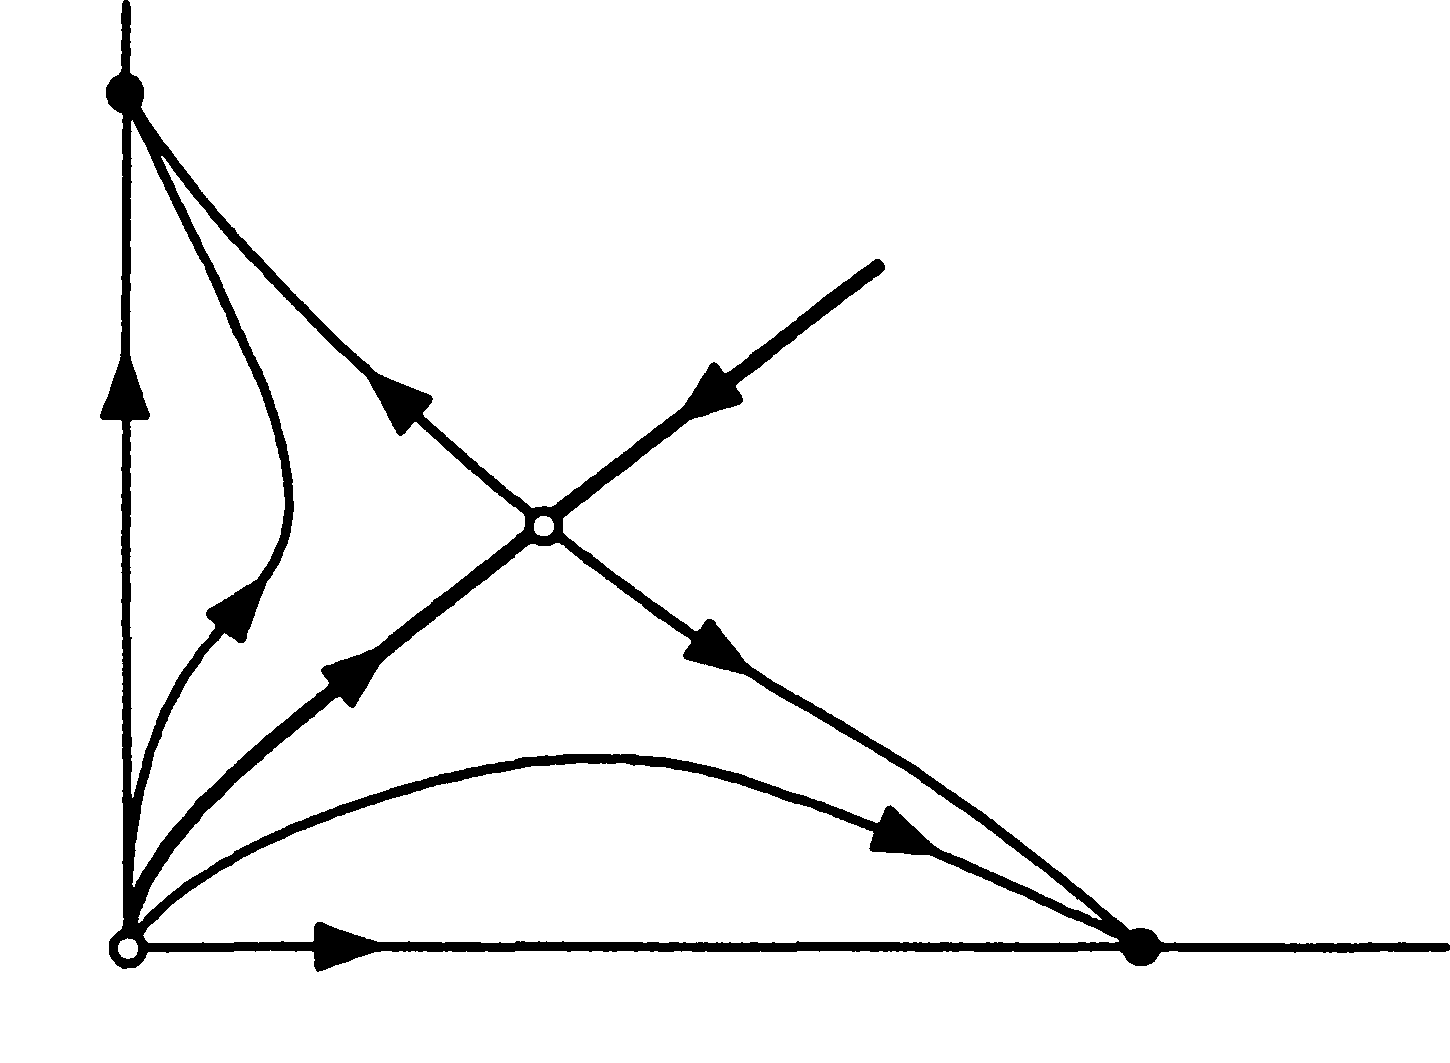
\includegraphics[width=0.82\textwidth]{images/Figures/figur-014.png}
\caption{Eyerin kararlı manifoldu ile tamamlanan faz portresi taslağı.}
\label{fig:6-4-6}
\end{figure}
\begin{figure}[H]
\centering
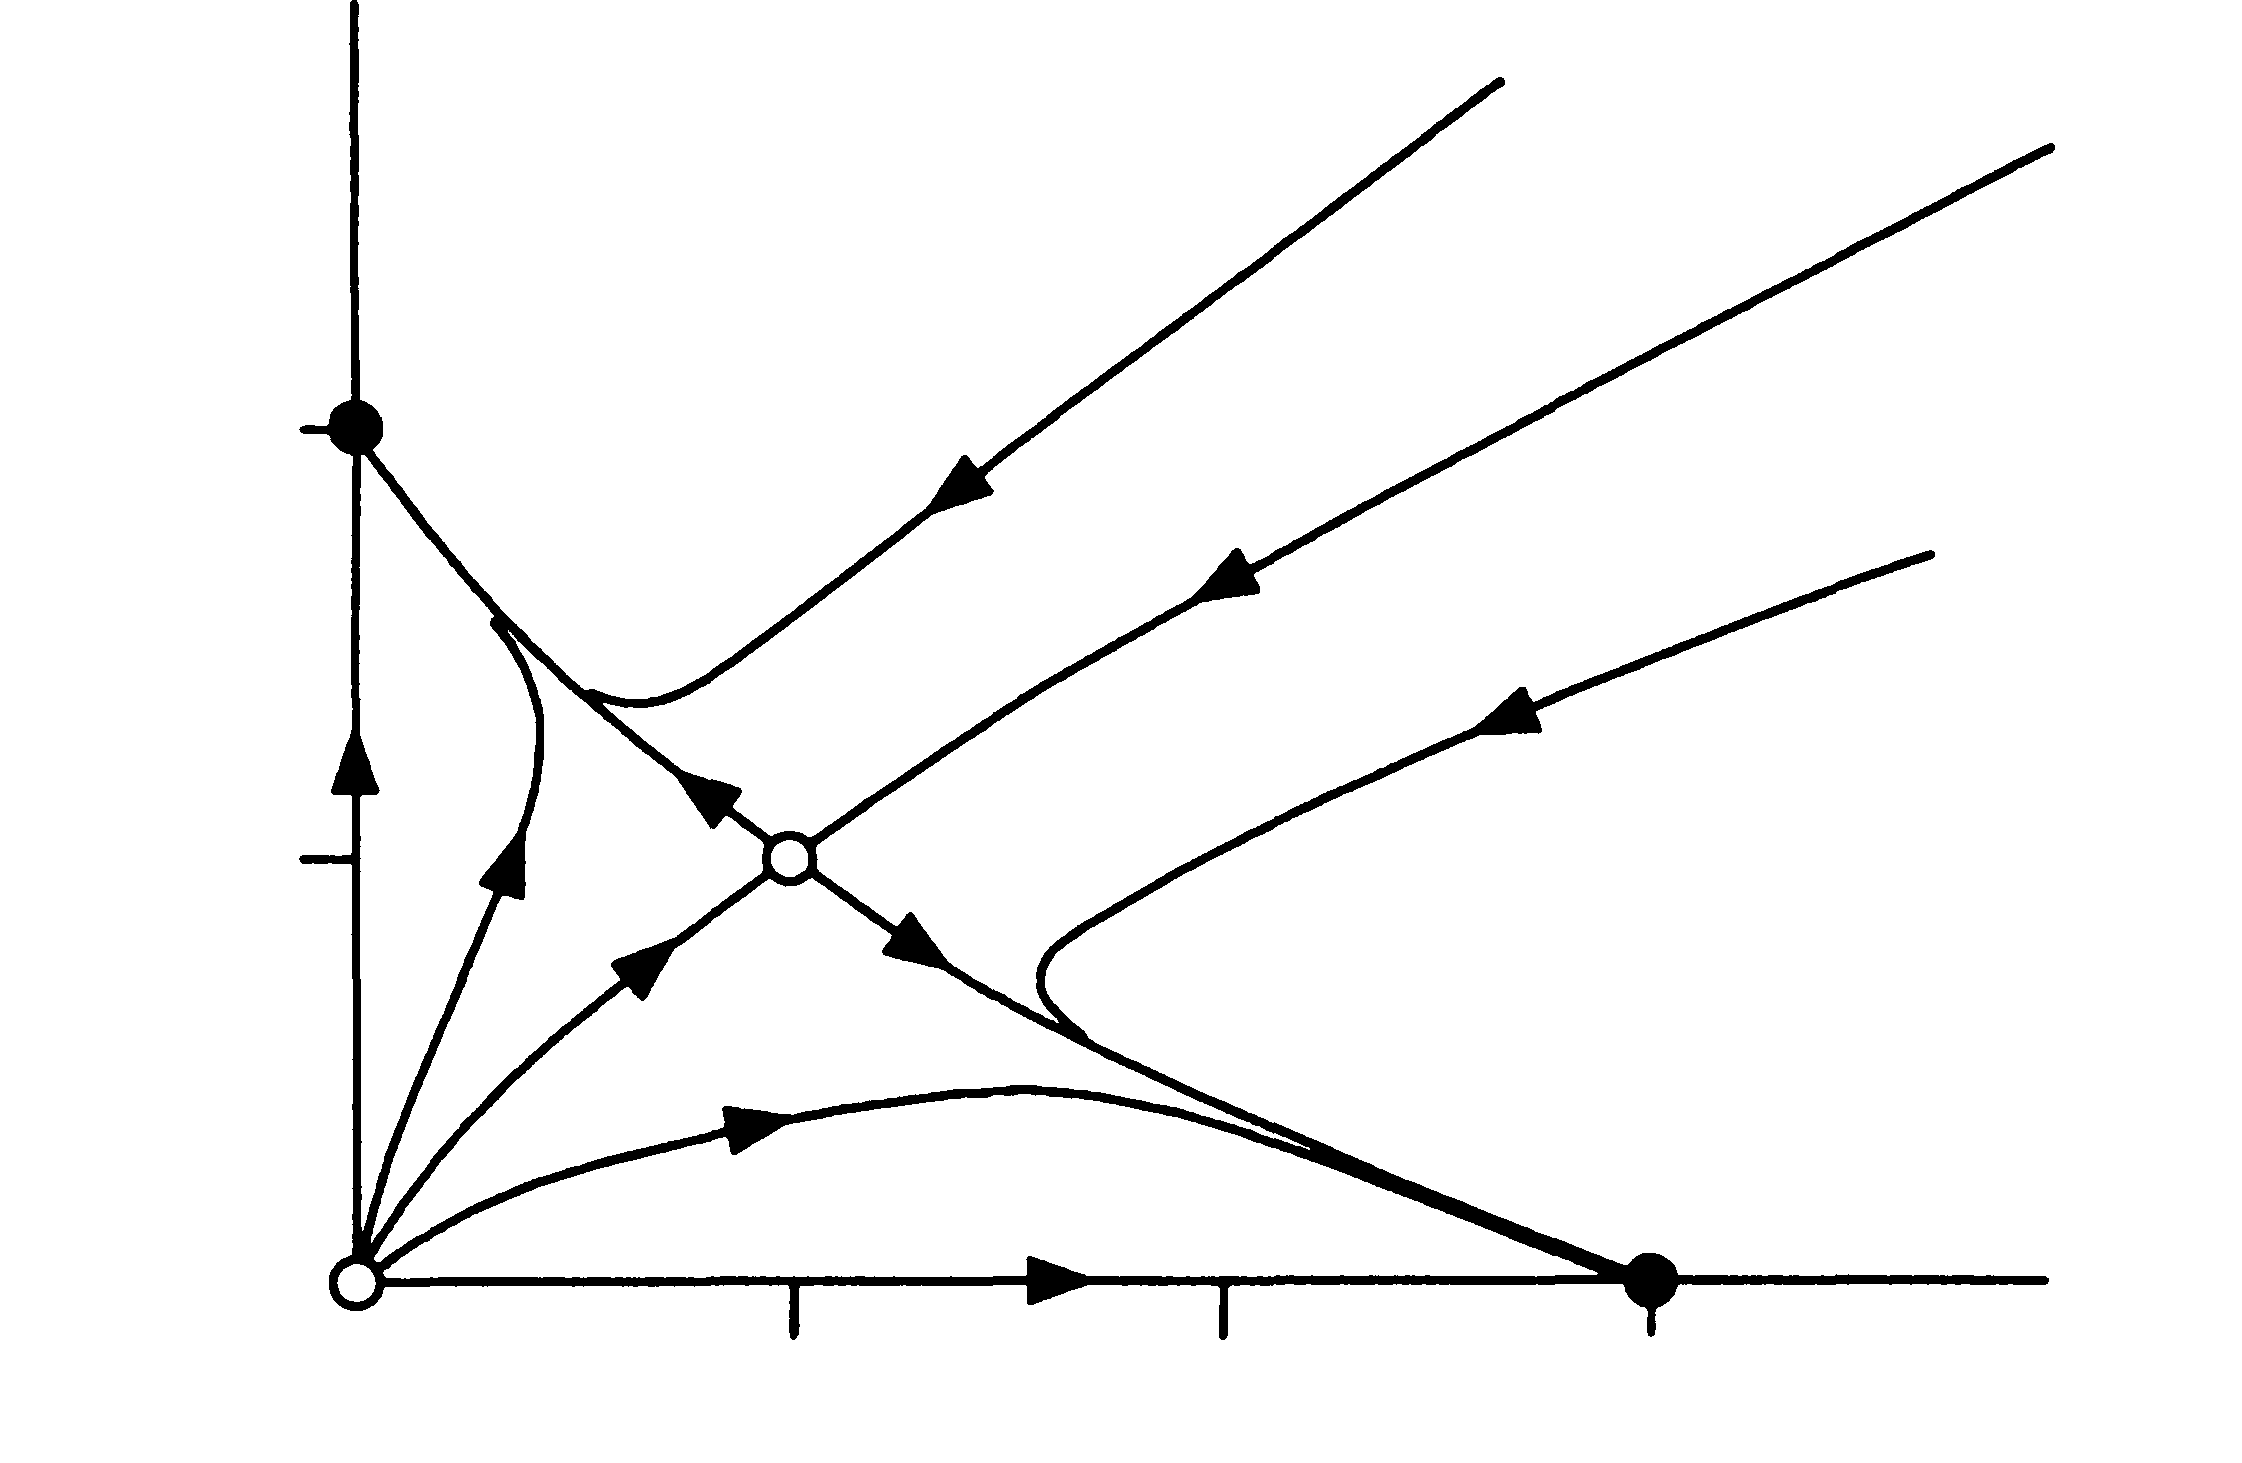
\includegraphics[width=0.82\textwidth]{images/Figures/figur-015.png}
\caption{Tavşan--koyun modeli için bilgisayar üretimli faz portresi.}
\label{fig:6-4-7}
\end{figure}

Biyolojik yorum şudur: Kararlı manifoldun altında başlayan yörüngeler koyunların, üstünde başlayan yörüngeler ise tavşanların yok oluşuna yol açar. Bu durum rekabetçi dışlama ilkesiyle ilişkilidir. $(3,0)$ düğümünün çekim havzası Şekil~\ref{fig:6-4-8}'de gösterilecektir.
\begin{figure}[H]
\centering
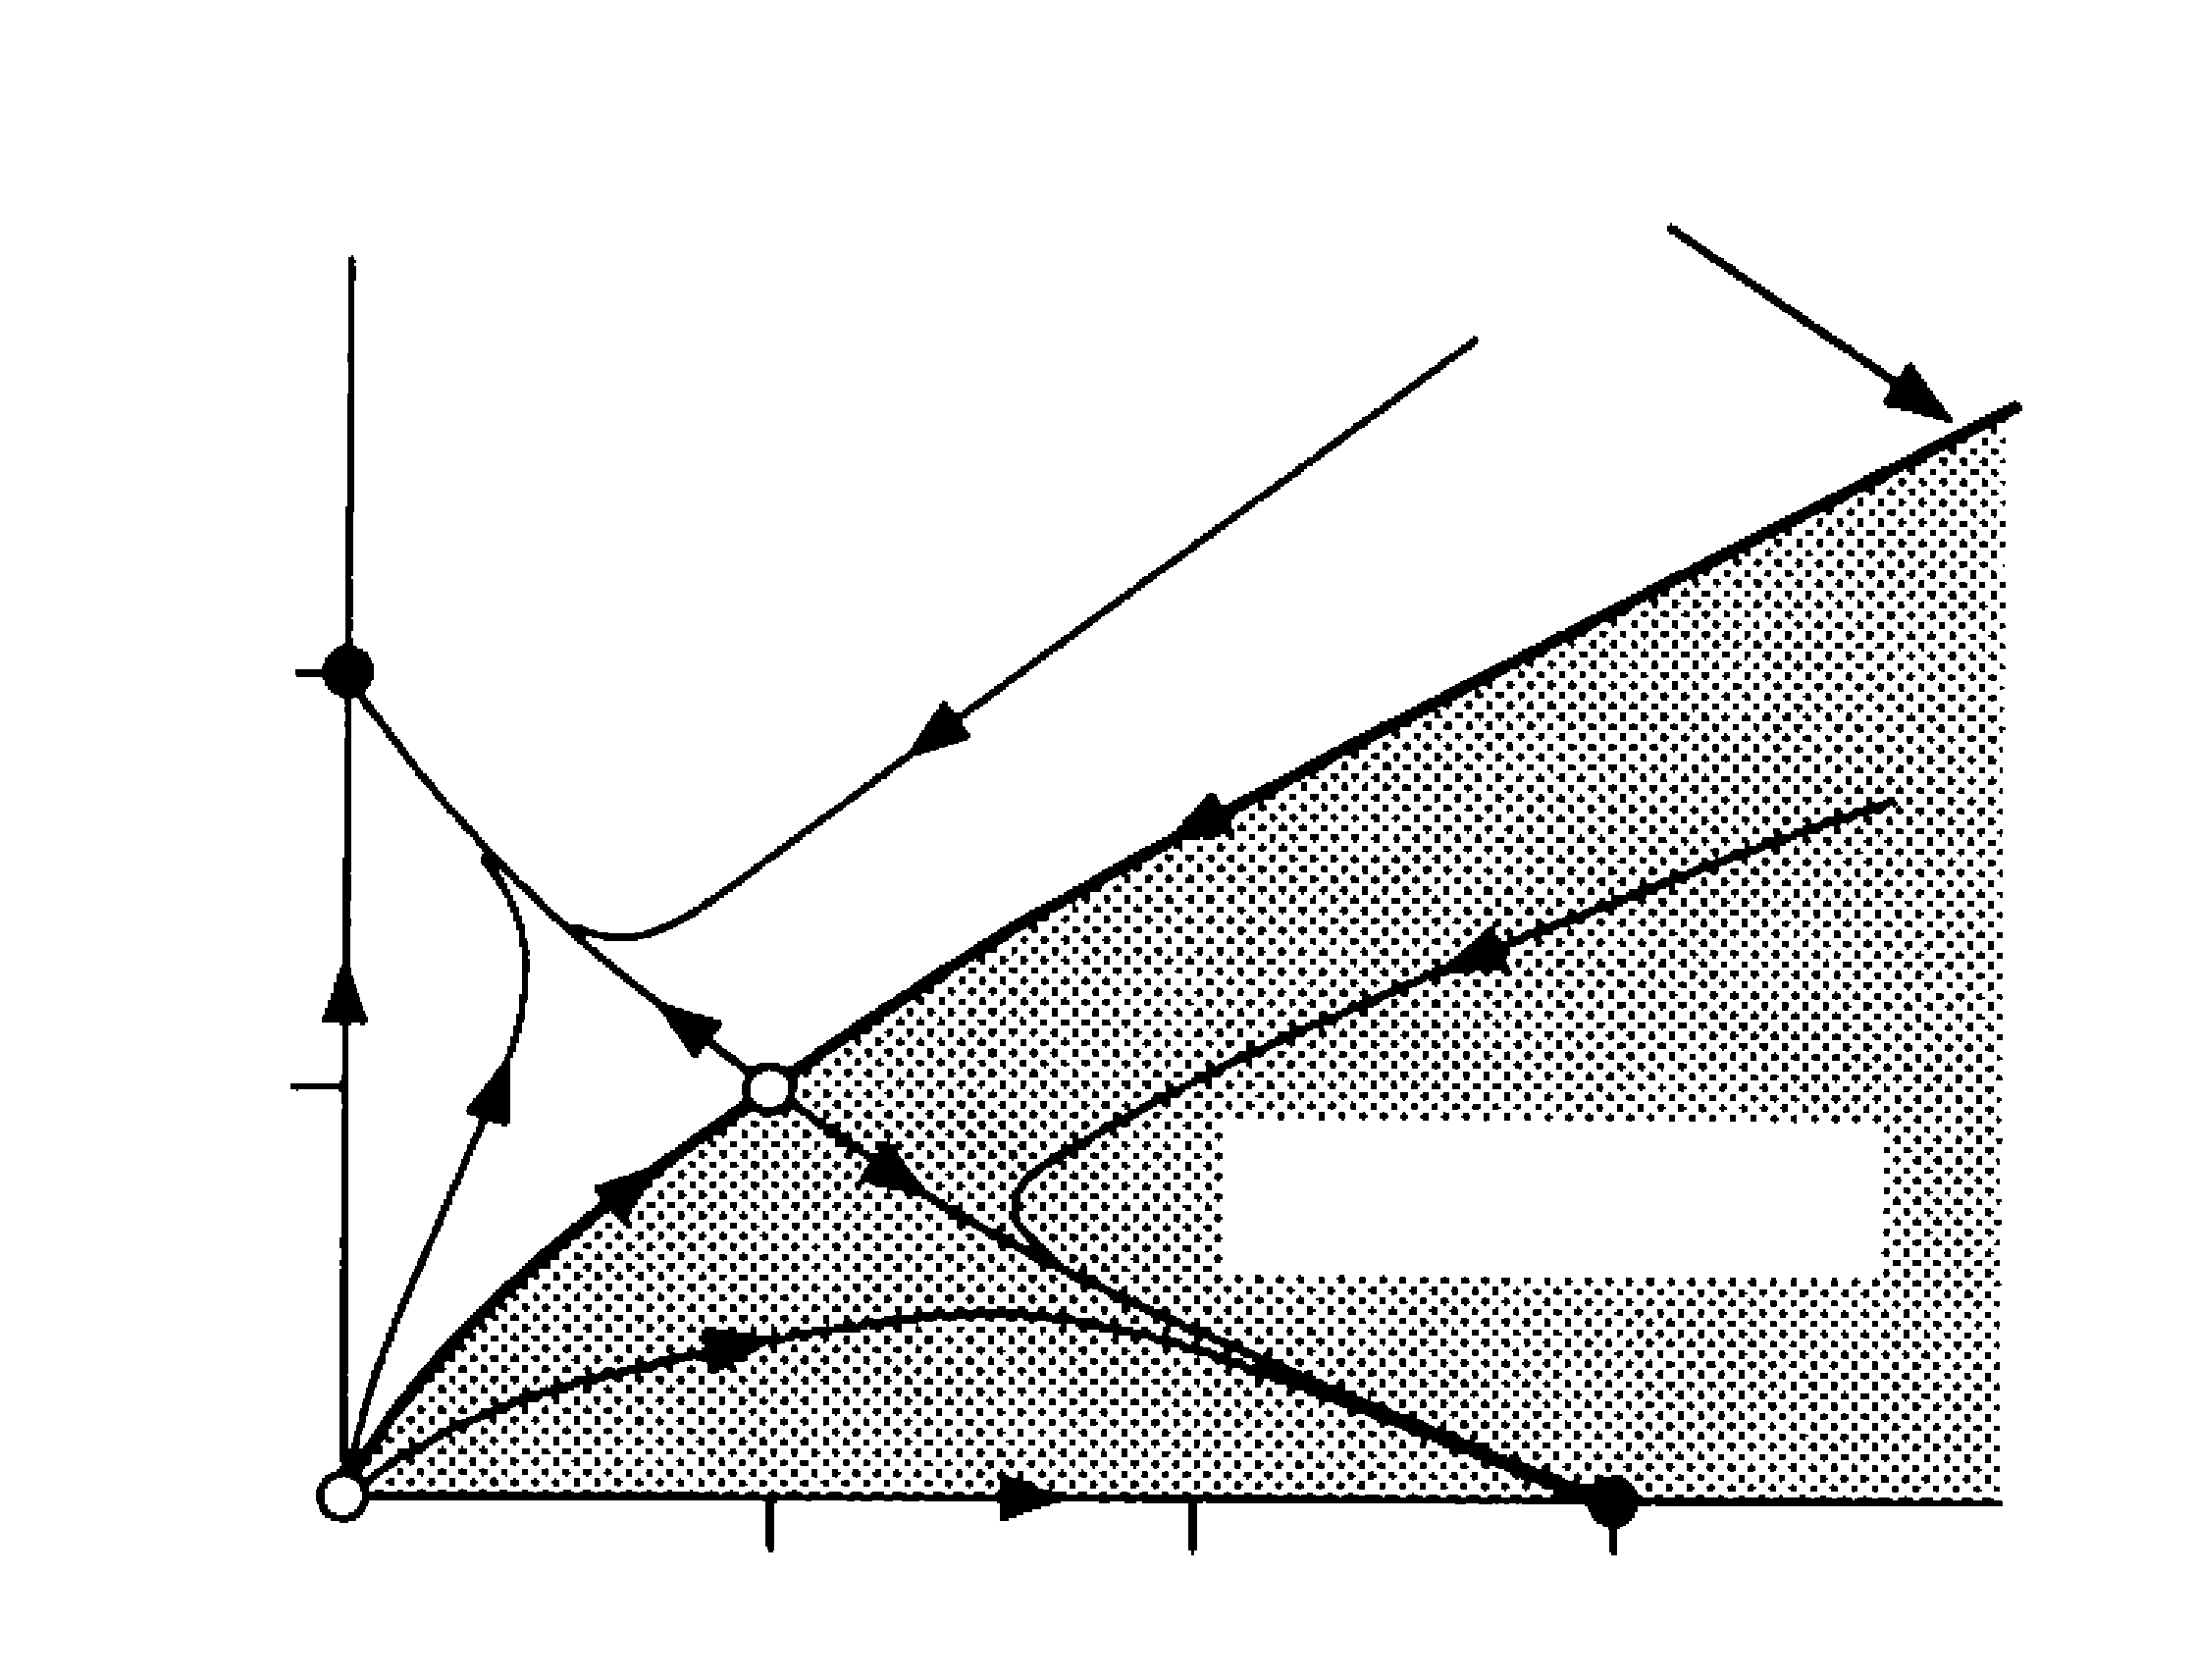
\includegraphics[width=0.82\textwidth]{images/Figures/figur-016.png}
\caption{$(3,0)$ noktasının çekim havzası ve havza sınırı.}
\label{fig:6-4-8}
\end{figure}
\end{justify}

\newpage